\documentclass{article}
\usepackage{hyperref}
\usepackage{listings}
\usepackage{color}
\usepackage{xcolor}
\usepackage{geometry}
\usepackage{graphicx}
\usepackage{amsmath}
\usepackage{caption}
\usepackage{subcaption}
\geometry{margin=1in}
\pdfminorversion=6

\newcommand\TODO[1]{\textcolor{red}{TODO: #1}}

\newcommand\header[2]{
    \begin{center}
        {\large
        UCSD CSE 168 Assignment #1: \\
        \vspace{0.3cm}
        \Large
        #2}
    \end{center}
}

\definecolor{dkgreen}{rgb}{0,0.6,0}
\definecolor{gray}{rgb}{0.5,0.5,0.5}
\definecolor{mauve}{rgb}{0.58,0,0.82}
\lstset{frame=tb,
        aboveskip=3mm,
        belowskip=3mm,
        showstringspaces=false,
        columns=flexible,
        basicstyle={\small\ttfamily},
        numbers=none,
        numberstyle=\tiny\color{gray},
        keywordstyle=\color{blue},
        commentstyle=\color{dkgreen},
        stringstyle=\color{mauve},
        breaklines=true,
        breakatwhitespace=true,
        tabsize=2
}

\hypersetup{colorlinks=true}


\begin{document}

\header{2}{Triangles and acceleration structures}

\begin{figure}[ht]
    \centering
    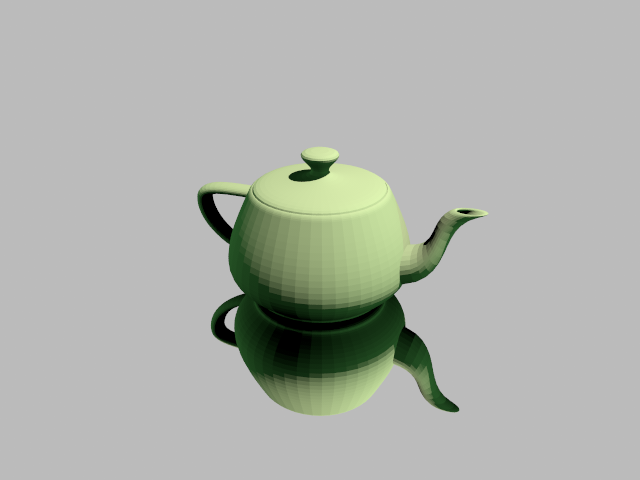
\includegraphics[width=0.20\linewidth]{imgs/hw_2_5a.png}
    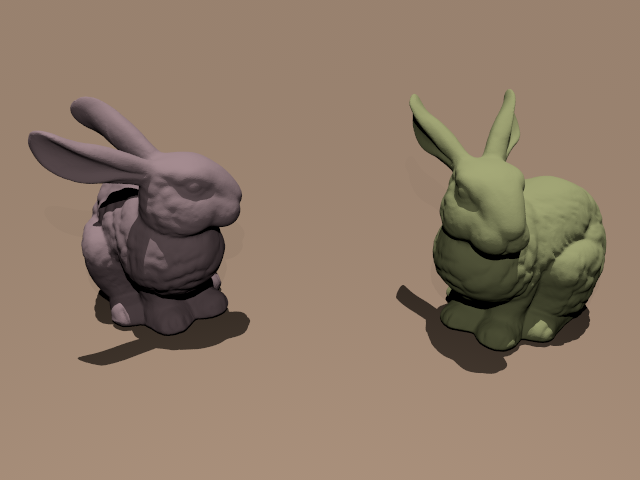
\includegraphics[width=0.20\linewidth]{imgs/hw_2_5b.png}
    \includegraphics[width=0.20\linewidth]{imgs/hw_2_5c.png}
    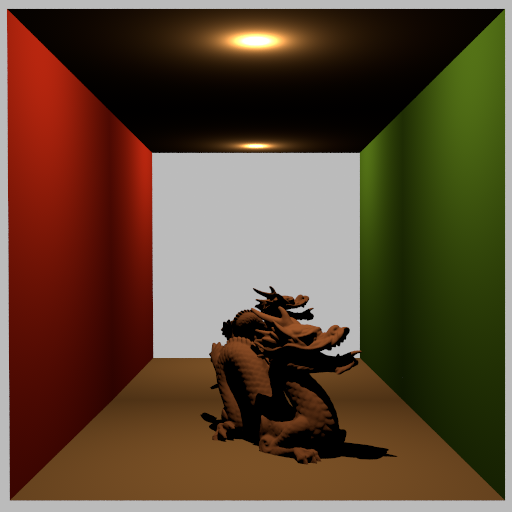
\includegraphics[width=0.15\linewidth]{imgs/hw_2_5d.png}
    \includegraphics[width=0.20\linewidth]{imgs/hw_2_5e.png}
    \caption{The images we will render in this homework.}
    \label{fig:teaser}
\end{figure}

In this homework, we are going to make your renderer capable of rendering more complex scenes (Figure~\ref{fig:teaser}).
The most commonly used primitive in computer graphics is a triangle. We will extend your renderer to handle objects that are made of \emph{triangle meshes}. Looping over each triangle for ray intersection is very slow. A scene can easily contain millions or billions of triangles (for example, in the movie Moana, \href{https://www.disneyanimation.com/resources/moana-island-scene/}{a scene of its island} contains more than 15 billion primitives). We will need something better.

For this homework, we will move to the second book of the Ray Tracing in One Weekend series: \href{https://raytracing.github.io/books/RayTracingTheNextWeek.html}{Ray Tracing - The Next Week (RTNW)}. As usual, we take huge inspirations from Wojciech Jarosz's \href{https://cs87-dartmouth.github.io/Fall2022/assignments.html}{CS 87/287 at Dartmouth}.

\section{Intersection with a single triangle (10 pts)}
Like our previous homework, let's start with rendering a single triangle. There are many ways to do it with different degrees of efficiency. The RTNW book did not provide information about triangles, but you can easily find some online. The \href{https://en.wikipedia.org/wiki/M%C3%B6ller%E2%80%93Trumbore_intersection_algorithm}{M\"oller-Trumbore intersection algorithm} described in the Wikipedia page is useful. The \href{https://www.pbr-book.org/3ed-2018/Shapes/Triangle_Meshes#TriangleIntersection}{PBRT book} contains more details.
Or you can just google ray-triangle intersection.
Feel free to copy paste any code.

Go to \lstinline{hw2.cpp} and look at the function \lstinline{hw_2_1}. Using the camera parameters provided (\lstinline{lookfrom = (0, 0, 0), lookat = (0, 0, -1), up = (0, 1, 0), vfov = 45}), render a triangle read from the command line arguments (we have parsed them for you). If your ray hits a triangle, outputs its barycentric coordinates (for a triangle $p_0, p_1, p_2$, a point inside the triangle can be represented as $p = w p_0 + u p_1 + v p_2$, where $(w, u, v)$ is the barycentric coordinate and $w = 1 - u - v$). Otherwise, if the ray does not hit anything, return $(0.5, 0.5, 0.5)$. To have consistency with our Homework 1 code, let's do antialiasing. We have parsed the \lstinline{-spp} argument for you too.

To see your results, type the following in the terminal:
\begin{lstlisting}[language=bash]
  ./torrey -hw 2_1 0  1 -3  -1 -1 -3  1 -1 -3
  ./torrey -hw 2_1 0  3 -4  -1 -2 -5  5 -1 -3
  ./torrey -hw 2_1 0 -3  1  -1  1 -4  1  1 -4
\end{lstlisting}

\begin{figure}[ht]
    \centering
    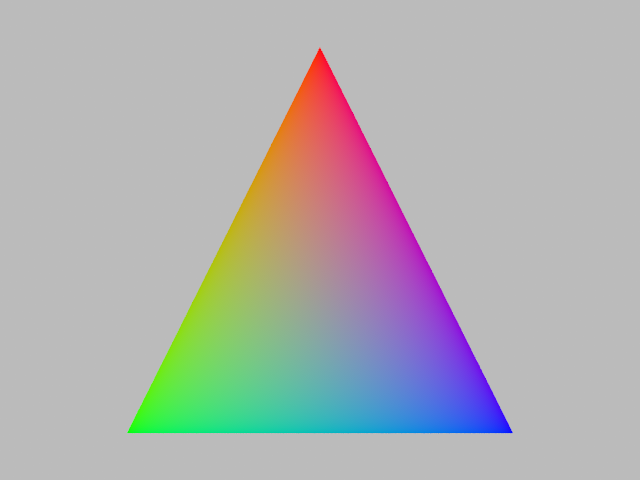
\includegraphics[width=0.3\linewidth]{imgs/hw_2_1a.png}
    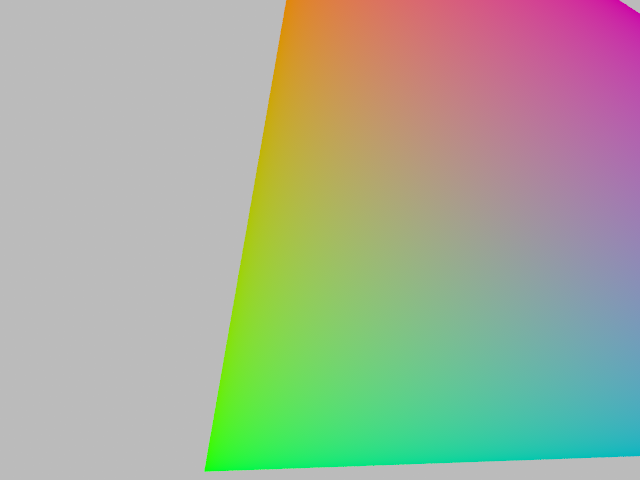
\includegraphics[width=0.3\linewidth]{imgs/hw_2_1b.png}
    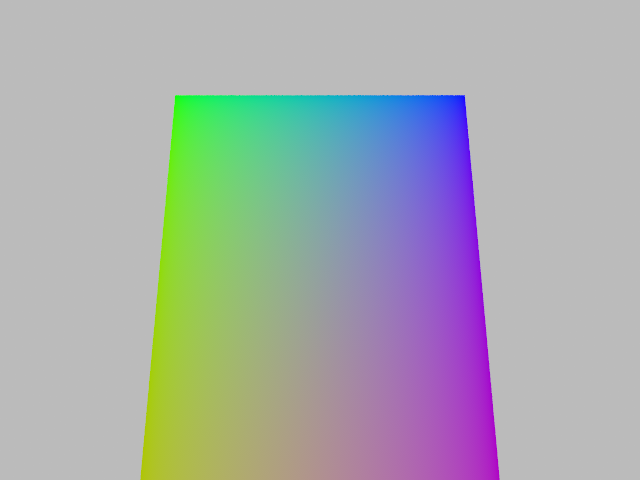
\includegraphics[width=0.3\linewidth]{imgs/hw_2_1c.png}
    \caption{References for Homework 2.1.}
    \label{fig:hw_2_1}
\end{figure}

\section{Intersection with a triangle mesh (10 pts)}
Let's extend the previous code to handle multiple triangles now. In computer graphics, we usually organize triangles in a \href{https://en.wikipedia.org/wiki/Triangle_mesh}{triangle mesh}. A triangle mesh consists of a list of \emph{vertices} which is just a bunch of 3D points, and a list of \emph{indices}, which connect the vertices into triangles. For example, following code represents a tetrahedron:
\begin{lstlisting}[language=C++]
    std::vector<Vector3> positions = {
        Vector3{ 0.0,  0.5, -2.0},
        Vector3{ 0.0, -0.3, -1.0},
        Vector3{ 1.0, -0.5, -3.0},
        Vector3{-1.0, -0.5, -3.0}
    };
    std::vector<Vector3i> indices = {
        Vector3i{0, 1, 2},
        Vector3i{0, 3, 1},
        Vector3i{0, 2, 3},
        Vector3i{1, 2, 3}
    };
\end{lstlisting}

Go to function \lstinline{hw_2_2} and extend your previous code to render the tetrahedron above. We will use the same camera pose, and we will again output the barycentric coordinates of the triangles. The \lstinline{-spp} argument is still there, but we don't need to touch it.

To see your results, type the following in the terminal:
\begin{lstlisting}[language=bash]
  ./torrey -hw 2_2
\end{lstlisting}

You should render something like Figure~\ref{fig:hw_2_2}.

\begin{figure}[ht]
    \centering
    \includegraphics[width=0.4\linewidth]{imgs/hw_2_2.png}
    \caption{References for Homework 2.2.}
    \label{fig:hw_2_2}
\end{figure}

\section{Parsing and rendering a scene. (30 pts)}
So far, we specify the scenes by either hardcoding them in code or we input a bunch of numbers in the command line. 
This is inconvienent. Usually, the input to a 3D rendering software is a text file describing a scene. It specifies the camera pose, lights, the materials of the objects, the geometry, and the rendering settings. There are many existing scene formats. For example see the \href{https://en.wikipedia.org/wiki/RenderMan_Interface_Specification}{RenderMan interface} and Pixar's \href{https://en.wikipedia.org/wiki/Universal_Scene_Description}{Universal Scene Description}. Here, we adopt the scene format from the \href{https://mitsuba.readthedocs.io/}{Mitsuba renderer}, simply because the scene file format is quite readable and there is an existing \href{https://github.com/mitsuba-renderer/mitsuba-blender}{Blender exporter}. We have provided the scene file parser for you, and you just need to convert the parsed information into your own data structure.

A typical Mitsuba scene is an XML file that looks like the following:
\begin{lstlisting}[language=xml]
<?xml version="1.0" encoding="utf-8"?>
<scene version="0.6.0">
  <sensor type="perspective">
    <string name="fovAxis" value="y"/>
    <transform name="toWorld">
      <lookAt origin="278, 273, -800" target="278, 273, -799" up="0, 1, 0"/>
    </transform>
    <float name="fov" value="39.3077"/>
    <sampler type="independent">
      <integer name="sampleCount" value="16"/>
    </sampler>
    <film type="hdrfilm">
      <integer name="width" value="512"/>
      <integer name="height" value="512"/>
    </film>
  </sensor>
  <!-- materials -->
  <bsdf type="diffuse" id="box">
    <rgb name="reflectance" value="0.884774, 0.699933, 0.666224"/>
  </bsdf>
  <bsdf type="diffuse" id="white">
    <rgb name="reflectance" value="0.884774, 0.699933, 0.666224"/>
  </bsdf>
  <bsdf type="diffuse" id="red">
    <rgb name="reflectance" value="0.56581, 0.0447145, 0.0441583"/>
  </bsdf>
  <bsdf type="diffuse" id="green">
    <rgb name="reflectance" value="0.105092, 0.378697, 0.0762035"/>
  </bsdf>
  <!-- lights -->
  <emitter type="point">
        <rgb name="intensity" value="1, 1, 1"/>
        <point name="position" x="278" y="548.8" z="279.5"/>
  </emitter>
  <!-- shapes -->
  <shape type="obj">
    <string name="filename" value="meshes/cbox_floor.obj"/>
    <ref id="white"/>
  </shape>
  <shape type="obj">
    <string name="filename" value="meshes/cbox_ceiling.obj"/>
    <ref id="white"/>
  </shape>
  <shape type="obj">
    <string name="filename" value="meshes/cbox_back.obj"/>
    <ref id="white"/>
  </shape>
  <shape type="obj">
    <string name="filename" value="meshes/cbox_greenwall.obj"/>
    <ref id="green"/>
  </shape>
  <shape type="obj">
    <string name="filename" value="meshes/cbox_redwall.obj"/>
    <ref id="red"/>
  </shape>
  <shape type="obj">
    <string name="filename" value="meshes/cbox_smallbox.obj"/>
    <ref id="box"/>
  </shape>
  <shape type="obj">
    <string name="filename" value="meshes/cbox_largebox.obj"/>
    <ref id="box"/>
  </shape>
  <background>
    <rgb name="radiance" value="0, 0, 0"/>
  </background>
</scene>
\end{lstlisting}

The whole scene is contained in a \lstinline{<scene>} tag. 
The scene is consists of \lstinline{sensor} (camera), \lstinline{bsdf} (materials), \lstinline{emitter} (lights), and \lstinline{shape} (geometry). 

The camera is specified as follows:
\begin{lstlisting}[language=xml]
  <sensor type="perspective">
    <string name="fovAxis" value="y"/>
    <transform name="toWorld">
      <lookAt origin="278, 273, -800" target="278, 273, -799" up="0, 1, 0"/>
    </transform>
    <float name="fov" value="39.3077"/>
    <sampler type="independent">
      <integer name="sampleCount" value="16"/>
    </sampler>
    <film type="hdrfilm">
      <integer name="width" value="512"/>
      <integer name="height" value="512"/>
    </film>
  </sensor>
\end{lstlisting}
We only support perspective cameras, and the \lstinline{transform} inside a sensor can only be a \lstinline{lookAt} transform. We only support \emph{independent} samplers, and inside it we specify the number of samples per pixel. We only support \lstinline{hdrfilm} which outputs an exr image with the specified width and height.

We can declare a list of materials and assign them to objects. A declaration looks like this:
\begin{lstlisting}[language=xml]
  <bsdf type="diffuse" id="box">
    <rgb name="reflectance" value="0.884774, 0.699933, 0.666224"/>
  </bsdf>
\end{lstlisting}
For this homework, you only need to support \lstinline{diffuse} and \lstinline{mirror} materials (just like the previous homework). In the future homeworks we will need to support more.

We can also declare a list of lights:
\begin{lstlisting}[language=xml]
  <emitter type="point">
        <rgb name="intensity" value="1, 1, 1"/>
        <point name="position" x="278" y="548.8" z="279.5"/>
  </emitter>
\end{lstlisting}
For this homework, you only need to support \lstinline{point} lights. In the future we will implement more lights.

Finally, we declare a list of shapes:
\begin{lstlisting}[language=xml]
  <shape type="obj">
    <string name="filename" value="meshes/cbox_floor.obj"/>
    <ref id="white"/>
  </shape>
\end{lstlisting}
A shape can be an \lstinline{obj} file, a \lstinline{ply} file, a \lstinline{serialized} file, a \lstinline{sphere}, or a \lstinline{rectangle}. An \href{https://en.wikipedia.org/wiki/Wavefront_.obj_file}{obj file} specifies a triangle mesh and looks like this:
\begin{lstlisting}
v 0 0 559.20001
v 0 0 0
v 0 548.79999 0
v 0 548.79999 559.20001
f 1 2 3 4
\end{lstlisting}
It specifies the 3D positions of vertices and the indices.

A \lstinline{ply} file is similar but stores the information in binary formats, making it more compact and efficient. Read the \href{https://en.wikipedia.org/wiki/PLY_(file_format)}{Wikipedia page} for more information.
\begin{lstlisting}[language=xml]
  <shape type="ply">
    <string name="filename" value="dragon.ply"/>
    <ref id="gold"/>
  </shape>
\end{lstlisting}

A \lstinline{serialized} file is Mitsuba's binary format.
\begin{lstlisting}[language=xml]
  <shape type="serialized">
    <string name="filename" value="sponza.serialized"/>
    <integer name="shapeIndex" value="29"/>
    <ref name="bsdf" id="sp_01_luk_a"/>
  </shape>
\end{lstlisting}

A shape can also be a sphere:
\begin{lstlisting}[language=xml]
  <shape type="sphere">
    <point name="center" x="1" y="2" z="3"/>
    <float name="radius" value="10"/>
    <ref id="white"/>
  </shape>
\end{lstlisting}
or a rectangle (converted to a triangle mesh with two triangles):
\begin{lstlisting}[language=xml]
  <shape type="rectangle">
    <!-- by default it is a rectangle spanning (-1, -1, 0) to (1, 1, 0) -->
    <ref id="gray"/>
  </shape>
\end{lstlisting}

The \lstinline{<ref>} tag references the materials we declared earlier and assign it to the shape. We can also declare the material inline as the following:
\begin{lstlisting}[language=xml]
  <shape type="sphere">
    <point name="center" x="1" y="2" z="3"/>
    <float name="radius" value="10"/>
    <bsdf type="diffuse">
      <rgb name="reflectance" value="0.5, 0.5, 0.5"/>
    </bsdf>
  </shape>
\end{lstlisting}

We can apply \emph{transformations} to shapes. The transformations supported are \lstinline{scale}, \lstinline{translate}, \lstinline{rotate}, \lstinline{lookat}, and \lstinline{matrix}. You specify it inside the shape:
\begin{lstlisting}[language=xml]
  <shape type="obj">
    <transform name="toWorld">
      <scale x="2" y="2" z="2"/>
      <translate x="5" y="6" z="7"/>
      <rotate angle="60" x="1" y="0" z="0"/>
      <matrix value="0 -0.53 0 -1.79 0.92 0 0 8.03 0 0 0.53 0 0 0 0 1"/>
    </transform>
    <string name="filename" value="meshes/cbox_floor.obj"/>
    <ref id="white"/>
  </shape>
\end{lstlisting}
We will apply the transformations in order. The matrix transform specifies the transformation in row-major order.
The transformation is only supported with \lstinline{obj} and \lstinline{ply}. You can't transform a sphere (we just want to make things simpler -- it is actually easy to implement transformed spheres).

Finally, we can specify the color of the background when a ray doesn't hit an object:
\begin{lstlisting}[language=xml]
  <background>
    <rgb name="radiance" value="0, 0, 0"/>
  </background>
\end{lstlisting}
(This syntax was not in original Mitsuba, I made this to fit better to our scenes).

After passing the xml file into our parser (using the \lstinline{parse_scene} function defined in \lstinline{parse_scene.h} and \lstinline{parse_scene.cpp}), it returns a \lstinline{ParsedScene}:
\begin{lstlisting}[language=C++]
struct ParsedScene {
    ParsedCamera camera;
    std::vector<ParsedMaterial> materials;
    std::vector<ParsedLight> lights;
    std::vector<ParsedShape> shapes;
    Vector3 background_color;
    int samples_per_pixel;
};
\end{lstlisting}
where \lstinline{ParsedCamera} is defined as:
\begin{lstlisting}[language=C++]
struct ParsedCamera {
    Vector3 lookfrom;
    Vector3 lookat;
    Vector3 up;
    Real vfov;
    int width, height;
};
\end{lstlisting}
\lstinline{ParsedMaterial} is defined as:
\begin{lstlisting}[language=C++]
struct ParsedDiffuse {
    ParsedColor reflectance;
};
struct ParsedMirror {
    ParsedColor reflectance;
};
// ...
using ParsedMaterial = std::variant<ParsedDiffuse, ParsedMirror, /* ... */>;
\end{lstlisting}
\lstinline{ParsedLight} is defined as:
\begin{lstlisting}[language=C++]
struct ParsedPointLight {
    Vector3 position;
    Vector3 intensity;
};
// ...
using ParsedLight = std::variant<ParsedPointLight, /* ... */>;
\end{lstlisting}
\lstinline{ParsedShape} is defined as:
\begin{lstlisting}[language=C++]
struct ParsedShapeBase {
    int material_id = -1;
    int area_light_id = -1;
};
struct ParsedSphere : public ParsedShapeBase {
    Vector3 position;
    Real radius;
};
struct ParsedTriangleMesh : public ParsedShapeBase {
    std::vector<Vector3> positions;
    std::vector<Vector3i> indices;
    std::vector<Vector3> normals;
    std::vector<Vector2> uvs;
};
using ParsedShape = std::variant<ParsedSphere, ParsedTriangleMesh>;
\end{lstlisting}
and \lstinline{ParsedColor} is defined as:
\begin{lstlisting}[language=C++]
using ParsedColor = std::variant<Vector3 /* RGB */, /* ... */>;
\end{lstlisting}

There is a bit of information to unpack. \lstinline{ParsedCamera} should be straightforward.
\lstinline{ParsedMaterial}, \lstinline{ParsedLight}, and \lstinline{ParsedShape} are defined using 
C++17 feature \lstinline{std::variant}. It's basically a \emph{tagged union} that encapsulates:
\begin{lstlisting}[language=C++]
struct Foo {
  int type;
  union {
    Type0 t0;
    Type1 t1;
    // ...
  }
};
\end{lstlisting}
Read more about it \href{https://www.cppstories.com/2020/04/variant-virtual-polymorphism.html/}{here}.

You do not need to worry about area lights.
You do not need to worry about \lstinline{normals} and \lstinline{uvs} in \lstinline{ParsedTriangleMesh}.
You do not need to worry about \lstinline{ParsedImageTexture}.
We will implement all of these in Homework 3.

What you need to do is to render the scenes we provide using your renderer in the function \lstinline{hw_2_3}. This should mostly just be converting the parsed data structure into your own data structures. 
We have provided scenes that reproduce the ones you rendered in Homework 1. 
We also provided a few new ones that contains triangle meshes.

This part of the homework is a bit tedious and slightly involved. We provide here the constructor of our own scene data structure that converts a \lstinline{ParsedScene} into our scene. You do not have to follow this:
\begin{lstlisting}[language=C++]
struct Scene {
    Scene(const ParsedScene &scene);

    Camera camera;
    int width, height;
    std::vector<Shape> shapes;
    std::vector<Material> materials;
    std::vector<Light> lights;
    Vector3 background_color;

    int samples_per_pixel;
    // For the Triangle in the shapes to reference to.
    std::vector<TriangleMesh> meshes;
};

Scene::Scene(const ParsedScene &scene) :
        camera(from_parsed_camera(scene.camera)),
        width(scene.camera.width),
        height(scene.camera.height),
        background_color(scene.background_color),
        samples_per_pixel(scene.samples_per_pixel) {
    // Extract triangle meshes from the parsed scene.
    int tri_mesh_count = 0;
    for (const ParsedShape &parsed_shape : scene.shapes) {
        if (std::get_if<ParsedTriangleMesh>(&parsed_shape)) {
            tri_mesh_count++;
        }
    }
    meshes.resize(tri_mesh_count);

    // Extract the shapes
    tri_mesh_count = 0;
    for (int i = 0; i < (int)scene.shapes.size(); i++) {
        const ParsedShape &parsed_shape = scene.shapes[i];
        if (auto *sph = std::get_if<ParsedSphere>(&parsed_shape)) {
            shapes.push_back(
                Sphere{{sph->material_id, sph->area_light_id},
                    sph->position, sph->radius});
        } else if (auto *parsed_mesh = std::get_if<ParsedTriangleMesh>(&parsed_shape)) {
            meshes[tri_mesh_count] = TriangleMesh{
                {parsed_mesh->material_id, parsed_mesh->area_light_id},
                parsed_mesh->positions, parsed_mesh->indices,
                parsed_mesh->normals, parsed_mesh->uvs};
            // Extract all the individual triangles
            for (int face_index = 0; face_index < (int)parsed_mesh->indices.size(); face_index++) {
                shapes.push_back(Triangle{face_index, &meshes[tri_mesh_count]});
            }
            tri_mesh_count++;
        } else {
            assert(false);
        }
    }

    // Copy the materials
    for (const ParsedMaterial &parsed_mat : scene.materials) {
        if (auto *diffuse = std::get_if<ParsedDiffuse>(&parsed_mat)) {
            // We assume the reflectance is always RGB for now.
            materials.push_back(Diffuse{std::get<Vector3>(diffuse->reflectance)});
        } else if (auto *mirror = std::get_if<ParsedMirror>(&parsed_mat)) {
            // We assume the reflectance is always RGB for now.
            materials.push_back(Mirror{std::get<Vector3>(mirror->reflectance)});
        } else {
            assert(false);
        }
    }

    // Copy the lights
    for (const ParsedLight &parsed_light : scene.lights) {
        // We assume all lights are point lights for now.
        ParsedPointLight point_light = std::get<ParsedPointLight>(parsed_light);
        lights.push_back(PointLight{point_light.intensity, point_light.position});
    }
}
\end{lstlisting}
Note that we convert a triangle mesh into many triangle primitives. This will make the later part of the homework much easier, and we recommend you to do so too:
\begin{lstlisting}[language=C++]
struct Triangle {
    int face_index;
    const TriangleMesh *mesh;
};
\end{lstlisting}

To see your results, type the following in the command line:
\begin{lstlisting}[language=bash]
./torrey -hw 2_3 [scene_filename]
\end{lstlisting}
For example, if you are in the build directory, \lstinline{./torrey -hw 2_3 ../scenes/hw1_spheres/scene0.xml} would render a scene from Homework 1.

Test your code in the following scenes: 
\begin{itemize}
  \item \lstinline{scenes/hw1_spheres/scene0.xml} to \lstinline{scenes/hw1_spheres/scene4.xml} are the scenes from the previous homework, and you should get the exact same results. 
  \item \lstinline{scenes/hw2_triangles/single_triangle.xml} and \lstinline{scenes/hw2_triangles/tetrahedron.xml} are the two scenes above.
  \item \lstinline{scenes/cbox/cbox_point_light.xml} and \lstinline{scenes/cbox/cbox_point_light_spheres.xml} renders into images in Figure~\ref{fig:hw_2_3}.
\end{itemize}

\begin{figure}[ht]
    \centering
    \includegraphics[width=0.3\linewidth]{imgs/hw_2_3a.png}
    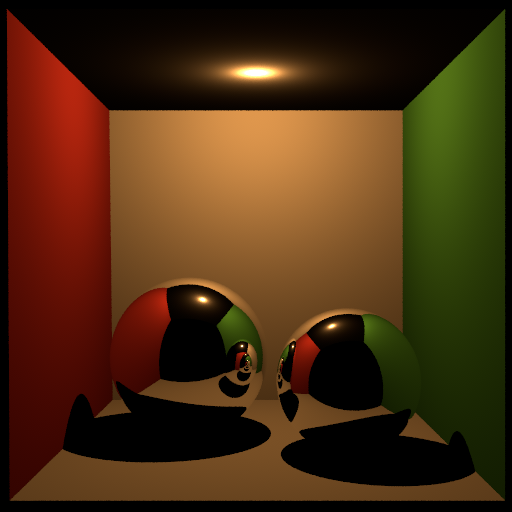
\includegraphics[width=0.3\linewidth]{imgs/hw_2_3b.png}
    \caption{References for Homework 2.3.}
    \label{fig:hw_2_3}
\end{figure}

\section{Intersection with axis-aligned bounding boxes (10 pts)}
So far we have only rendered scenes with relatively small amount of primitives. It would be cool if we can render more complex scenes, but our current way to handle ray-scene intersection would not scale to a high number of primitives. To improve this, we will implement an \emph{acceleration data structure}. The one we will implement in this homework is the \emph{bounding volume hierarchy} -- it's the most popular one in  modern ray tracers. We will use axis-aligned bounding boxes as our bounding volumes -- they are shown to be very fast to intersect with and provide a relatively tight bounds for our primitives. Thus, a crucial component of a typical bounding volume hierarchy is the intersection between rays and axis aligned bounding boxes. 

In this part, we will implement the intersection routine between a ray and an axis-aligned bounding box. First, read \href{https://raytracing.github.io/books/RayTracingTheNextWeek.html#boundingvolumehierarchies}{Chapters 3.1 to 3.6} of RTNW and understand the content.

Next, go to function \lstinline{hw_2_4} and modify the code. Your code should take a scene as an input just like in Homework 2.3. You will construct an axis-aligned bounding box for each sphere and each triangle. You will next intersect the camera rays against these boxes. If the ray hits any of the boxes, outputs the color $(1, 1, 1)$, otherwise outputs the color $(0.5, 0.5, 0.5)$.

\paragraph{Degenerated axis-aligned bounding boxes.}
The ray-AABB intersection code provided in the RTNW book has a slight issue which will cause problem when rendering axis-aligned bounding boxes that have exactly zero length in one dimension. The code looks like this:
\begin{lstlisting}[language=C++]
inline bool aabb::hit(const ray& r, double t_min, double t_max) const {
    for (int a = 0; a < 3; a++) {
        auto invD = 1.0f / r.direction()[a];
        auto t0 = (min()[a] - r.origin()[a]) * invD;
        auto t1 = (max()[a] - r.origin()[a]) * invD;
        if (invD < 0.0f)
            std::swap(t0, t1);
        t_min = t0 > t_min ? t0 : t_min;
        t_max = t1 < t_max ? t1 : t_max;
        if (t_max <= t_min)
            return false;
    }
    return true;
}
\end{lstlisting}
The problem is in the line \lstinline{if (t_max <= t_min)}: if a bounding box has the same \lstinline{min()[a]} and \lstinline{max()[a]}, it would result in \lstinline{t_min == t_max} and a ray would never intersect with the box. The solution is simple: just change it to \lstinline{if (t_max < t_min)}.

Use the scene \lstinline{scenes/aabb_test/aabb_test.xml} to test your rendering. As usual, type the following:
\begin{lstlisting}[language=bash]
./torrey -hw 2_4 [scene_filename]
\end{lstlisting}
If you use your Homework 2.3 code to render it, it will look like the left on Figure~\ref{fig:hw_2_4}. If you use your Homework 2.4 code to render it, it will look like the right.

\begin{figure}[ht]
    \centering
    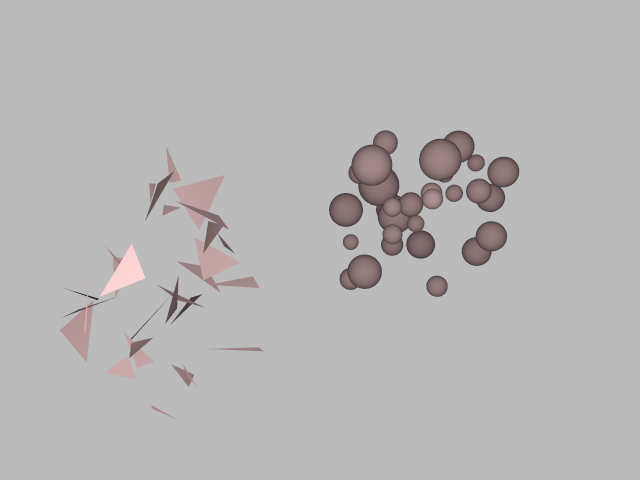
\includegraphics[width=0.3\linewidth]{imgs/hw_2_4a.png}
    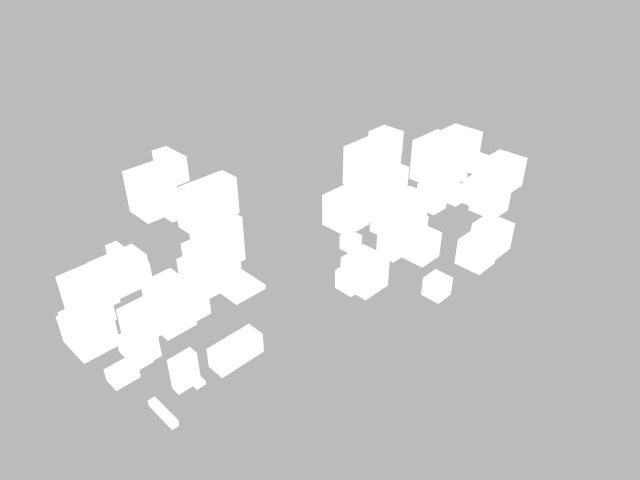
\includegraphics[width=0.3\linewidth]{imgs/hw_2_4b.png}
    \caption{References for Homework 2.4.}
    \label{fig:hw_2_4}
\end{figure}

\section{Bounding volume hierarchies (30 pts)}
We're going to implement the real deal now. This will finally allow us to render more complex scenes. As mentioned in the RTNW book, the idea is to build a tree of the axis-aligned bounding boxes, traverse the tree with a given ray, and skip a whole branch of tree if the ray does not intersect with the box. 

Read through \href{https://raytracing.github.io/books/RayTracingTheNextWeek.html#boundingvolumehierarchies/creatingboundingboxesoflistsofobjects}{Chapter 3.7 to 3.10} of RTNW. Go to \lstinline{hw_2_5} and implement your BVH renderer (use the same shading as Homework 2.3). It should not change the results of all your previous renderings.

We provide a few more scenes for you to test your algorithms. The models are from the \href{https://graphics.stanford.edu/data/3Dscanrep/}{Stanford 3D Scanning Repository} and from \href{https://casual-effects.com/data/}{Morgan Mcguire's Computer Graphics Archive}. The \lstinline{teapot} has 15704 triangles, the \lstinline{bunny} has 144046 triangles, the \lstinline{buddha} has 1087474 triangles, the \lstinline{dragon} has 871306 triangles, and the \lstinline{armadillo} has 212574 triangles. Imagine how long it would take to render these scenes if you don't have a BVH!

\paragraph{Quiz: choosing the axis to divide in BVH construction (3 pts).} The RTNW book recommended to split the BVH by randomly choosing an axis. Another popular strategy is to choose the axis with the largest extent. Experiment both and let us know which one is faster for you.

\paragraph{ProgressReporter and Timer.} From now on, the scenes in the homeworks can take longer to render. To assist you to judge how long it takes to render a scene, we provide two classes for showing the rendering progress and the rendering time. The \lstinline{ProgressReporter} prints out the percentage of completion of a task and the \lstinline{Timer} is a wrapper around the modern C++ \lstinline{std::chrono} library. See the comments for how to use them in \lstinline{progress_reporter.h} and \lstinline{timer.h}.

To test your rendering on these scenes, type (assuming you are in \lstinline{torrey/build} directory):
\begin{lstlisting}[language=bash]
./torrey -hw 2_5 ../scenes/teapot/teapot_constant.xml
./torrey -hw 2_5 ../scenes/bunny/bunny.xml
./torrey -hw 2_5 ../scenes/buddha/buddha.xml
./torrey -hw 2_5 ../scenes/dragon/dragon.xml
./torrey -hw 2_5 ../scenes/party/party.xml
\end{lstlisting}

You should render images like the ones in Figure~\ref{fig:hw_2_5}. On my 2019 MacBook Pro (with a 2.6 GHz 6-Core Intel Core i7), the BVH took around 1-5 seconds to build for these scenes, and the rendering itself takes a couple seconds.
\begin{figure}[ht]
    \centering
    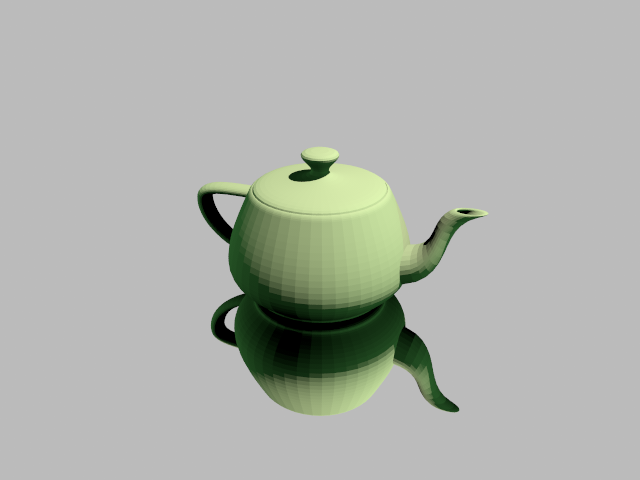
\includegraphics[width=0.20\linewidth]{imgs/hw_2_5a.png}
    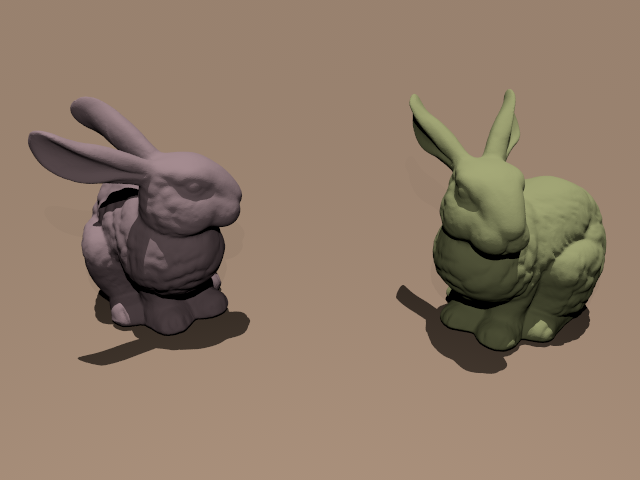
\includegraphics[width=0.20\linewidth]{imgs/hw_2_5b.png}
    \includegraphics[width=0.20\linewidth]{imgs/hw_2_5c.png}
    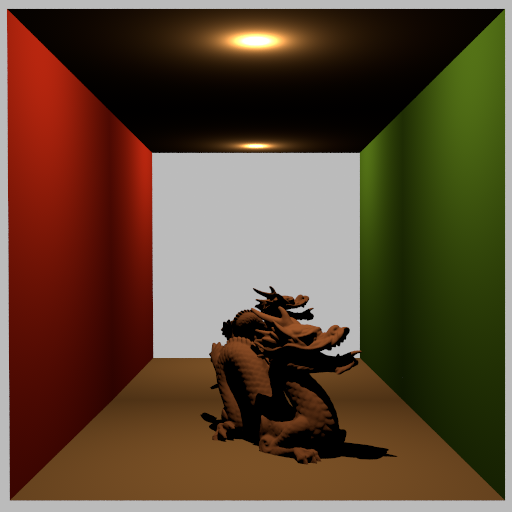
\includegraphics[width=0.15\linewidth]{imgs/hw_2_5d.png}
    \includegraphics[width=0.20\linewidth]{imgs/hw_2_5e.png}
    \caption{References for Homework 2.5.}
    \label{fig:hw_2_5}
\end{figure}

\section{Design your own scene (10 pts)}
We've come to the usual fun part of the homework! Design a scene yourself and render it. Feel free to download models on the internet (we recommend converting them to \lstinline{.ply} instead of \lstinline{.obj} since our obj parser is very slow). 

You can either manually author a \lstinline{.xml} scene (maybe start by modifying an existing one), or use the \href{https://github.com/mitsuba-renderer/mitsuba-blender}{Mitsuba Blender add-on} to convert a scene in Blender to the Mitsuba scene format. Note that the converter does not support all Blender features, and we do not support all features in the Mitsuba scene format, so you likely still need some manual editing before and after the conversion.

\section{Bonus: speedup your BVH code (30 pts)}
The basic BVH we implemented above would not be the most efficient BVH out there. In this optional part, you would explore ways to make your BVH code faster. Here are a few ideas for you:
\begin{itemize}
  \item Implement the \href{https://www.pbr-book.org/3ed-2018/Primitives_and_Intersection_Acceleration/Bounding_Volume_Hierarchies#TheSurfaceAreaHeuristic}{surface area heuristic} for building a better BVH.
  \item Parallelizing the BVH construction.
  \item Compactifying the BVH node data structure (e.g., do we need to store three integers?).
  \item During the BVH traversal, visit the closer bounding volume first (see the \href{https://www.pbr-book.org/3ed-2018/Primitives_and_Intersection_Acceleration/Bounding_Volume_Hierarchies#Traversal}{PBRT} book for an explanation).
  \item Instead of a binary tree, build a n-ary tree and make use of SIMD instructions (see \href{http://www.cs.cmu.edu/afs/cs/academic/class/15869-f11/www/readings/wald08_widebvh.pdf}{Wald et al.'s paper} for more information).
  \item Use \lstinline{std::nth_element} instead of \lstinline{std::sort} when building the BVH.
\end{itemize}

In a report, document what have you tried and benchmark your speedup (measure both BVH construction and rendering, exclude parsing).
Let the total speedup ratio be $c$, your score for the bonus would be $\min(c \cdot 10, 30)$ (i.e., if you achieve a 3x speedup, you get the full bonus points).
To make it fair for people with different kinds of machines, please measure your speedup using 2 threads by adding \lstinline{-t 2} in command line.

\section{Bonus: motion blur (15 pts)}
Read \href{https://raytracing.github.io/books/RayTracingTheNextWeek.html#motionblur}{Chapter 2} of RTNW and implement motion blur in your renderer. You may need to hack into the scene parser to parse scenes with different geometric transforms at different time instances.

\section{Bonus: object instancing (15 pts)}
Read \href{https://raytracing.github.io/books/RayTracingTheNextWeek.html#instances}{Chapter 8} of RTNW and implement object instancing in your renderer.

%\bibliographystyle{plain}
%\bibliography{refs}

\end{document}
